\documentclass{article}
\usepackage{titling}
\usepackage{titlesec}
\usepackage[margin=3.45cm]{geometry}
\usepackage{graphicx}
\usepackage{subcaption}

\setlength{\droptitle}{-2cm}
\titleformat{\section}
  {\normalfont\Large\bfseries}{\thesection}{1em}{}

\title{\textbf{Mapping the Journey - An Exploratory Study of Road Safety in Great Britain}}
\author{Bhanu Prakash Bhaskarla}
\date{\today}

\begin{document}

\maketitle

% Abstract
\section{Abstract}
This survey provides a detailed exploration through an Exploratory Data Analysis (EDA) of road safety data,
with a specific emphasis on incidents involving personal injuries in Great Britain throughout the year 2019.
The statistical insights presented herein are exclusively derived from incidents that transpired on public
roads, leading to personal injuries. These incidents were reported to the police and meticulously documented
through the STATS19 accident reporting form, ensuring a comprehensive and standardized record of each occurrence.
The utilization of such a structured reporting mechanism facilitates a nuanced examination of the circumstances
surrounding each incident, enhancing the depth and precision of the ensuing exploratory data analysis. This study
is initially carried out after removing all the missing values and inconsistencies from the dataset as part of the
initial exploration and for the second iteration of analysis, the outliers in the data are also removed.

\noindent\textbf{Keywords:} Road Safety, Exploratory Data Analysis, Data Visualization, Correlation Analysis,
Outlier Detection.

% Contents
\section{Contents}
The report is organized as follows:
\begin{enumerate}
  \item Introduction
  \item Data Preprocessing
  \item Data Visualization
  \item Correlation Analysis
  \item Outlier Detection
  \item Conclusion
  \item Bibliography
\end{enumerate}

% Introduction
\section{Introduction}
Making sure that roads are safe is a very important goal for governments around the world. The information about
road accidents in Great Britain for the year 2019 includes 117,536 individual records, each with 32 different
details. It's important to know that all the information in this set is coded, meaning it's not written out in
regular words.
This study takes a close look at the data we just mentioned. The Department for Transport of Great Britain is the
group that puts together, organizes, and shares this important information about transportation safety.
This study lets us explore many different parts of road safety in a detailed way. It gives us helpful information
to make smart decisions and create rules for safety in transportation.
The programming language used for this study is Python. The libraries used are Pandas, NumPy, Matplotlib, Seaborn,
and GeoPandas.

\textbf{Features:}
Accident\_Index, Location\_Easting\_OSGR, Location\_Northing\_OSGR, Longitude, Latitude,
Police\_Force, Accident\_Severity, Number\_of\_Vehicles, Number\_of\_Casualties, Date,
Day\_of\_Week, Time, Local\_Authority\_(District), Local\_Authority\_(Highway), 1st\_Road\_Class,
1st\_Road\_Number, Road\_Type, Speed\_limit, Junction\_Detail, Junction\_Control, 2nd\_Road\_Class,
2nd\_Road\_Number, Pedestrian\_Crossing-Human\_Control, Pedestrian\_Crossing-Physical\_Facilities,
Light\_Conditions, Weather\_Conditions, Road\_Surface\_Conditions, Special\_Conditions\_at\_Site,
Carriageway\_Hazards, Urban\_or\_Rural\_Area, Did\_Police\_Officer\_Attend\_Scene\_of\_Accident,
LSOA\_of\_Accident\_Location.

% Data Preprocessing
\section{Data Preprocessing}
Data preprocessing is a crucial step in the road safety exploratory data analysis (EDA) process. It involves
cleaning and transforming the raw road safety dataset into a structured and usable format for analysis. The
goal is to address issues such as missing values, inconsistencies, ensuring the dataset is reliable and suitable
for deriving meaningful insights. The following subsections describe the data preprocessing steps undertaken.

\subsection{Handling Missing Values}
Missing values in the attributes of the dataset are as follows:
\begin{enumerate}
  \item Location\_Easting\_OSGR: 28
  \item Location\_Northing\_OSGR: 28
  \item Longitude: 28
  \item Latitude: 28
  \item Time: 63
  \item LSOA\_of\_Accident\_Location: 5,714
\end{enumerate}
Since the number of missing values are very less compared to the total number of records in the dataset, the
observations containing missing values are dropped from the dataset.

\subsection{Data Cleaning}
In the process of preparing for analysis, a critical step involves converting the 'Date'  and 'Time' columns to
the appropriate datetime format. This ensures consistency in the representation of temporal  data, allowing for
accurate and meaningful analysis. Moreover, Accident\_Index column is dropped from the dataset as it is not
necessary.

% Data Visualization
\section{Data Visualization}
In my quest to unravel insights from the road safety dataset, I employed a diverse set of data visualizations to
elucidate patterns, trends, and anomalies within the data. Visual representations not only enhance our understanding
but also provide a powerful means to communicate complex information. Let's delve into some key visualizations that
formed the cornerstone of our analysis.

\subsection{Distribution of Accident Severity}
Accident Severity is a critical metric that sheds light on the gravity of incidents. The following bar chart depicts
the number of accidents for each severity level. It is evident that the majority of accidents are of severity level
`3'(more than 80,000), followed by `2' and `1'.

\begin{figure}[ht]
  \centering
  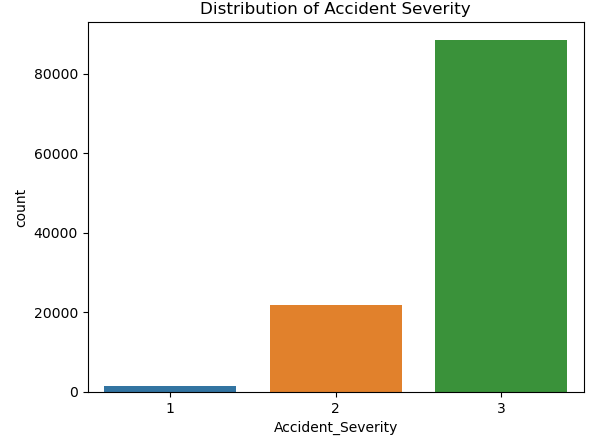
\includegraphics[width=0.5\textwidth]{Images/accident_severity.png}
  \caption{Distribution of Accident Severity}
\end{figure}

\subsection{Number of Accidents by hour of the day}
The analysis of accident patterns throughout the day unveils distinct temporal trends, guiding the formulation of
targeted road safety measures. Contrary to conventional morning rush hours, the data indicates a notable uptick in
accidents between 8:00 AM and 9:00 AM, aligning with increased commuting activity. Afternoons witness two
significant peaks, with the highest number of accidents occurring between 5:00 PM and 6:00 PM, followed by
another surge at 3:00 PM, coinciding with the conclusion of work and school hours. Evening hours demonstrate
a gradual decline, starting around 7:00 PM. Understanding these nuances provides a foundation for tailored
interventions during peak hours, emphasizing traffic management, visibility improvement, and safe driving
practices to enhance overall road safety.

\begin{figure}[ht]
  \centering
  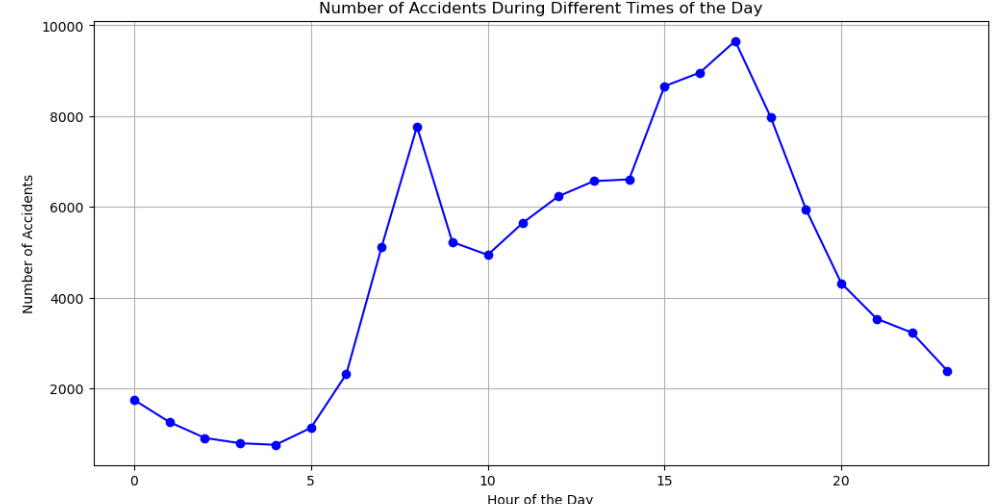
\includegraphics[width=0.5\textwidth]{Images/accidents_by_hour.png}
  \caption{Number of Accidents during differnt hours of the day}
\end{figure}

\subsection{Number of Accidents by day of the week}
Similarly, the analysis of accident patterns throughout the week reveals insights that can be leveraged to
formulate targeted road safety measures. The data indicates a notable uptick in accidents on Fridays, followed
by Thursdays and Wednesdays. The number of accidents is lowest on Sundays, followed by Saturdays.

\begin{figure}[ht]
  \centering
  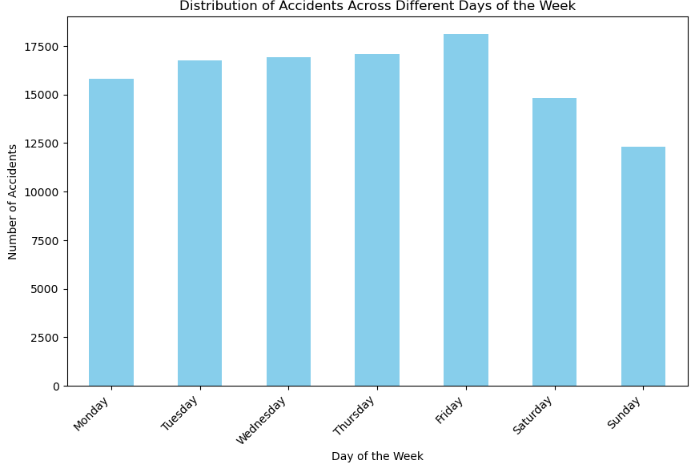
\includegraphics[width=0.5\textwidth]{Images/accidents_by_day.png}
  \caption{Number of Accidents during differnt days of the week}
\end{figure}

\subsection{Proportion of Accidents with Police Attendance}
The analysis of the dataset highlights the significant proportion of accidents attended by the police, a vital
aspect in evaluating emergency response effectiveness and overall road safety. This metric serves as a key
indicator of law enforcement involvement, impacting incident documentation, public safety, and thorough
investigations. Variations in police attendance across different accident severities, road types, and
urban/rural settings provide valuable insights.

\begin{figure}[ht]
  \centering
  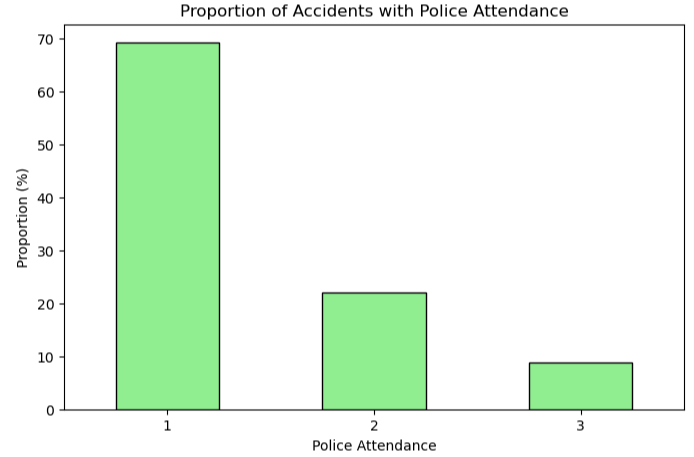
\includegraphics[width=0.5\textwidth]{Images/police_attendance.png}
  \caption{Proportion of Accidents with Police Attendance}
\end{figure}

\subsection{Geospatial Analysis}
Using latitude and longitude coordinates from the road safety dataset, I plotted the distribution of road accidents
across Great Britain. The GeoPandas library facilitated the creation of a GeoDataFrame, allowing for the seamless
integration of geographic information. The resulting map provides a visual representation of the geographical
concentration of road incidents, highlighting areas with elevated accident frequencies.

\begin{figure}[h]
  \centering
  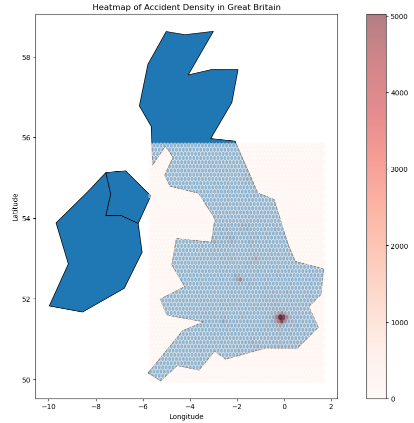
\includegraphics[width=0.5\textwidth]{Images/geographical_distribution.png}
  \caption{Geographical Distribution of Road Accidents}
\end{figure}

Beyond temporal patterns, the dataset offers a rich opportunity for insightful visualizations, providing a
comprehensive understanding of the factors influencing road safety. Two pivotal aspects, namely Weather
Conditions and Road Surface Conditions, significantly impact the occurrence and severity of accidents.

\begin{figure}[ht]
  \centering
  \begin{subfigure}{0.48\textwidth}
    \centering
    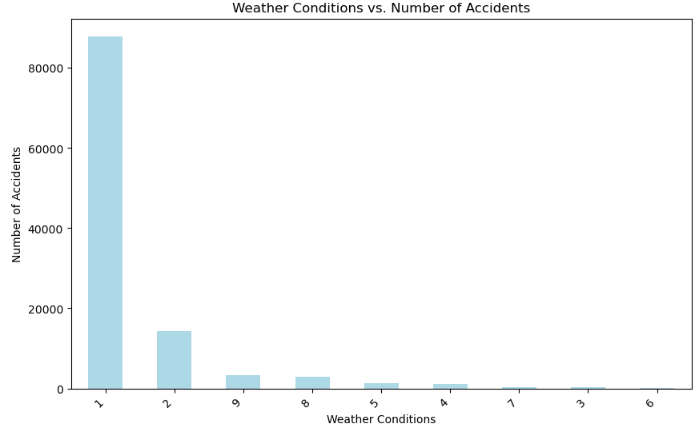
\includegraphics[width=\textwidth]{Images/weather_conditions.png}
    \caption{Weather Conditions}
  \end{subfigure}
  \hfill
  \begin{subfigure}{0.48\textwidth}
    \centering
    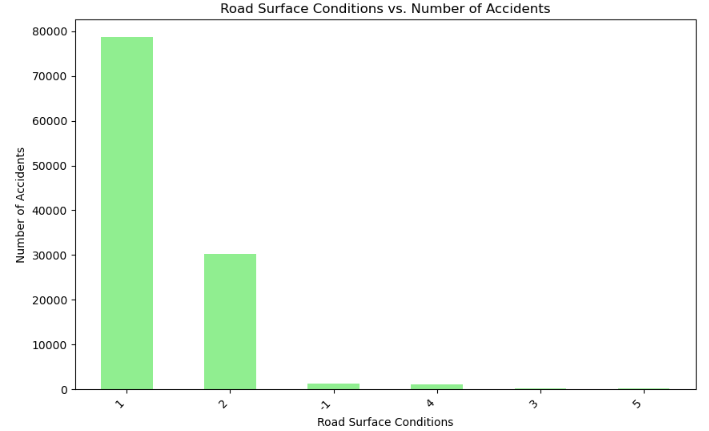
\includegraphics[width=\textwidth]{Images/road_surface_conditions.png}
    \caption{Road Surface Conditions}
  \end{subfigure}
  \caption{Impact of Weather and Road Surface Conditions on Road Safety}
\end{figure}

% Correlation Analysis
\section{Correlation Analysis}
Correlation analysis is a statistical technique that can show whether and how strongly pairs of variables are
related. For example, height and weight are related; taller people tend to be heavier than shorter people. The
relationship isn't perfect. But, on average, taller people are heavier. Correlation analysis in road safety EDA
explores relationships between variables, such as investigating how weather conditions correlate with accident
severity or how road surface conditions relate to the number of accidents. Utilizing correlation matrices and
visualizations provides insights into factors influencing road safety outcomes.

\subsection{Correlation Heatmap}
Dealing with a large number of features, the correlation matrix can indeed become congested, making it challenging
to interpret. To address this issue, I created a correlation matrix heatmap, highlighting the most significant
features.

\begin{figure}[ht]
  \centering
  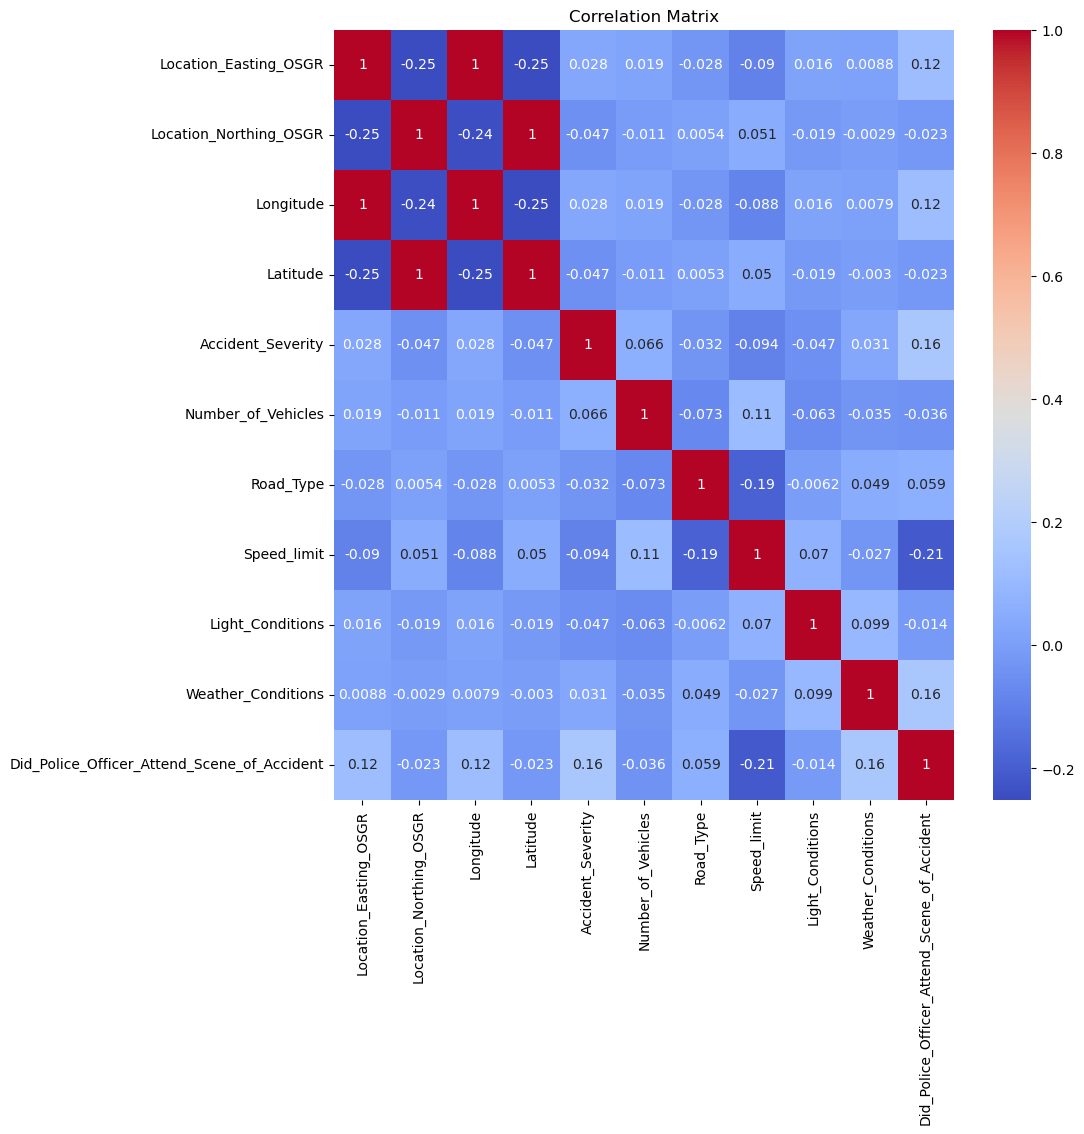
\includegraphics[width=1\textwidth]{Images/correlation_matrix.png}
  \caption{Correlation Matrix}
\end{figure}

% Outlier Detection
\section{Outlier Detection}
Outlier detection in road safety EDA involves identifying data points that significantly deviate from the norm,
offering valuable insights into exceptional incidents. Utilizing statistical methods like z-score analysis allows
for the pinpointing of anomalies, such as accidents with unusually high numbers of vehicles or casualties. By
isolating these outliers, the analysis can focus on understanding unique scenarios, contributing to a more
nuanced comprehension of road safety dynamics and potentially informing targeted interventions for specific
outlier-driven patterns.

\subsection{Outlier Detection using Z-Score for Number of Casualties}
The z-score is the signed number of standard deviations by which the value of an observation or data point is
above the mean value of what is being observed or measured. Threshold for z-score is set to `3'.

\begin{figure}[ht]
  \centering
  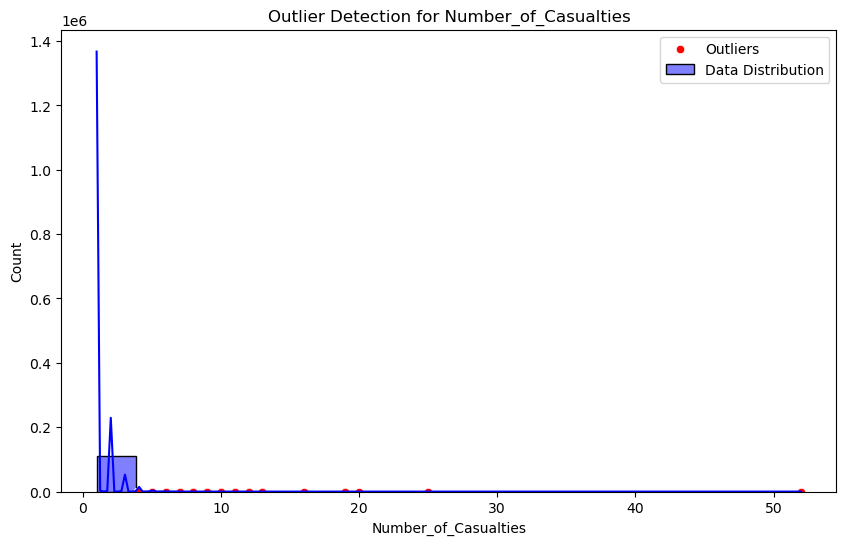
\includegraphics[width=0.5\textwidth]{Images/outlier_detection.png}
  \caption{Outlier Detection using Z-Score for Number of Casualties}
\end{figure}

% Conclusion
\section{Conclusion}
The road safety dataset offers a rich opportunity for exploratory data analysis, providing a comprehensive
understanding of the factors influencing road safety. The analysis of temporal patterns, geographical
concentration, and correlation matrices provides valuable insights into the dynamics of road safety in Great
Britain.

\subsection{Iterative Analysis}
The process of Exploratory Data Analysis (EDA) in the context of road safety is inherently iterative, reflecting
the dynamic nature of the data exploration journey. By employing a cyclical approach, analysts can unravel the
complexities of road safety datasets more comprehensively. The second iteration of analysis involves the removal
of outliers from the dataset, facilitating a more nuanced understanding of the factors influencing road safety.
For those seeking predictive insights, iterative EDA is crucial for refining models. Each iteration allows for
the adjustment of model parameters, feature selection, and validation, ensuring that the predictive models
evolve in response to the identified patterns. As insights unfold, new questions and hypotheses may arise.
Iterative EDA allows for the continuous refinement of these questions, ensuring that the analysis remains
aligned with the evolving understanding of the road safety landscape. Here are the key insights from the
second iteration of analysis:

\begin{enumerate}
  \item The dataset contains 80825 records after removing the outliers.
  \item Distribution of Accident Severity
\end{enumerate}

\begin{figure}[ht]
  \centering
  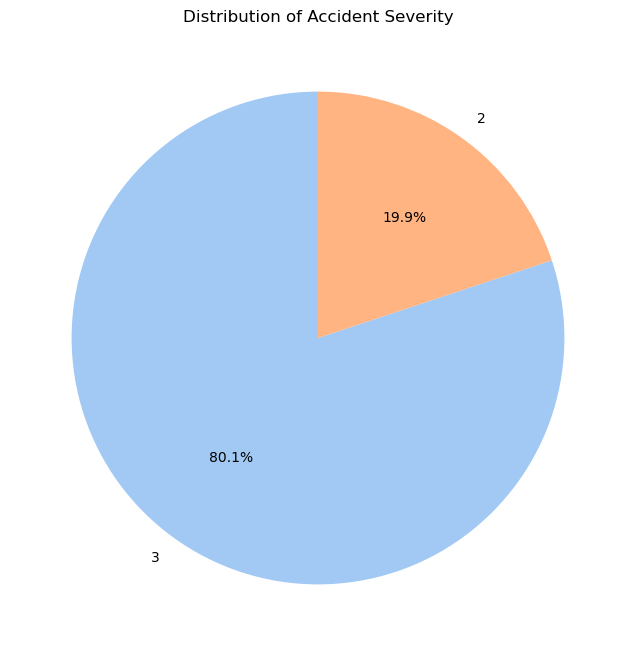
\includegraphics[width=0.5\textwidth]{Images/accident_severity_without_outliers.png}
  \caption{Accident Severity after removing outliers}
\end{figure}

\subsection{Hypothesis Testing}
Hypothesis testing is a statistical method that is used in making statistical decisions using experimental data.
Here, I have used the t-test to test the hypothesis that `There is no significant difference between the severity
of accidents in urban and rural areas'. The p-value is 1.3061220953688611e-61, which is less than the
significance level of 0.05. Hence, we reject the null hypothesis and conclude that there is a significant
difference between the severity of accidents in urban and rural areas.

% Bibliography
\section{Bibliography}
\begin{enumerate}
  \item \textbf{Road Safety Data} - \textit{https://www.kaggle.com/datasets/mostafafaramin/road-safety-data-accidents-2019/data}
  \item \textbf{GitHub} - \textit{https://github.com/bhanuprakash1606/road-safety-eda.git}
  \item \textbf{GeoPandas} - \textit{https://geopandas.org/}
  \item \textbf{Matplotlib} - \textit{https://matplotlib.org/}
  \item \textbf{Seaborn} - \textit{https://seaborn.pydata.org/}
  \item \textbf{Pandas} - \textit{https://pandas.pydata.org/}
  \item \textbf{NumPy} - \textit{https://numpy.org/}
\end{enumerate}

\end{document}